\chapter{牛顿运动定律}

\begin{introduction}
	\item \nameref{2.1}
	\item \nameref{2.2}
	\item \nameref{2.3}
	\item \nameref{2.4}
\end{introduction}

\section{牛顿运动定律} \label{2.1}

\subsection{牛顿第一定律}

\begin{axiom}[牛顿第一定律] \label{C2-ax1}
	任何质点都保持静止或者匀速直线运动状态, 直到其他物体对它作用的力迫使它改变这种状态为止. 
\end{axiom}

在实际应用中, 可以陈述为: 任何质点, 只要其他物体作用于它的所有力的合力为零, 则该质点就保持静止或者匀速直线运动状态不变. 

即合力$\va*{R} = \sum\limits_i \va*{F}_i = 0$, 其投影式为

\begin{equation}
	\begin{cases}
		R_x = \sum\limits_i F_{ix} = 0 \\
		R_y = \sum\limits_i F_{iy} = 0 \\
		R_z = \sum\limits_i F_{iz} = 0 
	\end{cases}
    \label{C2-eq1}
\end{equation}

\subsection{牛顿第二定律}

\begin{axiom}[牛顿第二定律] \label{C2-ax2}
	
	\begin{equation}
		\va*{R} = \sum\limits_i \va*{F}_i = \dv{(m\va*{v})}{t}
		\label{C2-eq2}
	\end{equation}
	
	某时刻质点动量对时间的变化率等于该时刻作用在质点上所有力的合力. 
	
	当质量可以看作常量时, 有
	
	\begin{equation}
		\va*{R} = \sum\limits_i \va*{F}_i = m \dv{\va*{v}}{t} = m \va*{a}
		\label{C2-eq3}
	\end{equation}
	
	力是一个物体对另一个物体的作用, 这种作用能迫使物体改变其运动状态, 即产生加速度. 
	
\end{axiom}

根据$\va*{a} = \dv{\va*{v}}{t} = \dv[2]{\va*{r}}{t}$, 式(\ref{C2-eq3})可以写为

\begin{equation}
	\va*{R} = \sum\limits_i \va*{F}_i = m \dv{\va*{v}}{t} = m \dv[2]{\va*{r}}{t}
	\label{C2-eq4}
\end{equation}

\newpage

投影到直角坐标系各坐标轴上, 可得

\begin{equation}
	\begin{cases}
		R_x = \sum\limits_i F_{ix} = m \dv{v_x}{t} = m \dv[2]{r_x}{t} \\
		R_y = \sum\limits_i F_{iy} = m \dv{v_y}{t} = m \dv[2]{r_y}{t} \\
		R_z = \sum\limits_i F_{iz} = m \dv{v_z}{t} = m \dv[2]{r_z}{t} 
	\end{cases}
    \label{C2-eq5}
\end{equation}

研究平面曲线运动时, 常用自然坐标

\begin{equation}
	\begin{cases}
		R_{\tau} = \sum\limits_i F_{i\tau} = m a_{\tau} = m \dv{v}{t} \\
		R_{n} = \sum\limits_i F_{in} = m a_{n} = m \frac{v^2}{\rho} 
	\end{cases}
    \label{C2-eq6}
\end{equation}

\subsection{牛顿第三定律}

\begin{axiom}[牛顿第三定律] \label{C2-ax3}
	当物体$A$以力$\va*{F}_1$作用于物体$B$时, 物体$B$也同时以$\va*{F}_2$作用于物体$A$上, 力$\va*{F}_2$和$\va*{F}_2$总是大小相等, 方向相反, 且在同一直线上. 
	
	\begin{equation}
		\va*{F}_1 = -\va*{F}_2 \label{C2-eq7}
	\end{equation}
	
\end{axiom}

\begin{note}
	
	作用力与反作用力有成对性和同时性. 但是牛顿第三定律适用于接触力, 对于非接触力则有延迟效应, 因为非接触力是通过场作用的, 场的传播速度是光速. 对于无施力者的力, 同样不适用牛顿第三定律. 
	
\end{note}

\section{常见的几种力} \label{2.2}

\subsection{万有引力}

\begin{equation}
	\va*{F}_{21} = G \dfrac{m_1 m_2}{r^2} \va*{r}^0
	\label{C2-eq8}
\end{equation}

其中, 引力常量$G = 6.67 \times 10^{-11} ~ \mathrm{m}^3 / (\mathrm{kg} \cdot \mathrm{s}^2)$, $\va*{r}^0$为一个由$m_1$指向$m_2$的单位矢量. 

地球对其表面附近尺寸不大的物体的万有引力, 近似等于该物体的重力. 

\begin{equation}
	P = G \dfrac{Mm}{R^2} = mg 
	\Longrightarrow g = G \dfrac{M}{R^2} \approx 9.8 \mathrm{m}/\mathrm{s}^2 
	\label{C2-eq9}
\end{equation}

\subsection{弹性力}

\begin{definition}[弹性力] \label{C2-df1}
	
	当两宏观物体有接触且发生微小形变时, 形变的物体对与它接触的物体会产生力的作用, 这种力叫弹性力. 
	
	在形变不超过一定限度内, 弹簧的弹性力遵从胡克定律
	
	\begin{equation}
		F_x = -kx \label{C2-eq10}
	\end{equation}
	
	其中, $k$为弹簧的劲度系数(曾称倔强系数). 
	
\end{definition}

\subsection{摩擦力}

\subsubsection{静摩擦力}

当两相互接触的物体彼此之间保持相对静止, 且沿接触面有相对运动趋势时, 在接触面之间会产生一对阻止上述运动趋势的力. 

静摩擦力的大小随引起相对运动趋势的外力而变化. 最大静摩擦力为

\begin{equation}
	f_{\mathrm{max}} = \mu_0 N \label{C2-eq11}
\end{equation}

其中, $\mu_0$为最大静摩擦系数, $N$为正压力. 

\subsubsection{滑动摩擦力}

两物体相互接触, 并有相对滑动时, 在两物体接触处出现的相互作用的摩擦力. 

\begin{equation}
	f = \mu N \label{C2-eq12}
\end{equation}

\subsubsection{流体阻力}

当物体穿过液体或气体运动时, 会受到流体阻力, 该阻力与运动物体速度方向相反, 大小随速度变化. 

\begin{enumerate}
	
	\item 当物体速度不太大时, 流体为层流, 阻力主要由流体的粘滞性产生. 这时流体阻力与物体速率成正比. 
	
	\begin{equation}
		f \propto v \label{C2-eq13}
	\end{equation}
	
	\item 当物体穿过流体的速率超过某限度时(低于声速), 流体出现旋涡, 这时流体阻力与物体速率的平方成正比. 
	
	\begin{equation}
		f \propto v^2 \label{C2-eq14}
	\end{equation}
	
	\item 当物体与流体的相对速度提高到接近空气中的声速时, 这时流体阻力将迅速增大. 
	
	\begin{equation}
		f \propto v^3 \label{C2-eq15}
	\end{equation}
	
\end{enumerate}

\section{牛顿运动定律的适用范围} \label{2.3}

\begin{definition}[惯性系、惯性力] \label{C2-df2}
	
	{\heiti 惯性系} 牛顿定律适用的参考系, 称为惯性系. 凡是相对惯性系作匀速直线运动的参考系也都是惯性系. 
	
	{\heiti 惯性力} 这是在非惯性系中应用牛顿第二定律引入的一种反映物体惯性的虚拟力. 以$\va*{a}_0$表示平动参考系的加速度, 则在此参考系中观测质点受的惯性力为
	
	\begin{equation}
		\va*{F}_i = -m \va*{a}_0 \label{C2-eq16}
	\end{equation}
	
\end{definition}

\section{第1次作业部分习题归纳} \label{2.4}

\subsection{运动学部分}

\subsubsection{基本概念明晰}

\begin{enumerate}
	
	\item (作业T3) 如果一个物体做匀速圆周运动, 则 \uline{物体是做变速运动}. 
	
	\vskip 0.1cm
	
	\begin{solution}
		$\bullet$ 做匀速圆周运动的物体, 速度、加速度、所受合力的大小都不变, 方向时刻在变化. 
	\end{solution}
	
	\vskip 0.3cm
	
	\item (作业T9) 曲线运动中, \uline{物体速度大小不一定变化, 速度方向一定变化, 一定具有加速度}. 
	
	\vskip 0.1cm
	
	\begin{solution}
		
		$\bullet$ 匀速圆周运动是曲线运动, 其速度大小不变.
		
		$\bullet$ 运动轨迹是曲线的运动是曲线运动, 做曲线运动的物体的速度的方向是沿切线方向, 方向一定变化. 
		
		$\bullet$ 速度方向改变就必须有法向加速度. 
		
	\end{solution}
	
\end{enumerate}

\subsubsection{运动学第一类问题(已知运动学方程, 通过求导, 求速度、加速度)}

\begin{enumerate}
	
	\item (作业T5) 作直线运动的质点的运动学方程为$x = 3t + 5t^3 - 6$, 则该质点作 \uline{变加速直线运动, 加速度沿$x$轴正向}. 
	
	\vskip 0.1cm
	
	\begin{solution}
		$\bullet$ 对运动学方程求两阶导得加速度$a = 30t$, 因为加速度$a$随时间$t$变化, 是变加速运动. 又$t \geqslant 0$, 则$a \geqslant 0$, 故加速度沿$x$轴正方向. 
	\end{solution}
	
	\vskip 0.3cm
	
	\item (作业T6) 质点在$y$轴上运动, 其运动方程为$y = 4t^2 - 2t^3$ (SI), 则质点返回原点时的 \uline{速度为$-8 \mathrm{~m}/\mathrm{s}$, 加速度为 $-16 \mathrm{~m}/\mathrm{s}^2$}. 
	
	\vskip 0.1cm
	
	\begin{solution}
		$\bullet$ 令$y = 0$, 解得质点返回原点的时间为$t = 2$ s($t = 0$舍去). 对该质点的运动方程求导得质点返回原点时速度$\eval{v}_{t=2} = \eval{8t - 6t^2}_{t=2} = -8 \mathrm{~m}/\mathrm{s}$, 再求导得$\eval{a}_{t=2} = \eval{8 - 12t}_{t=2} = -16 \mathrm{~m}/\mathrm{s}^2$. 
	\end{solution}
	
\end{enumerate}

\subsubsection{运动学第二类问题(已知速度、加速度, 结合初值条件积分求得运动学方程)}

\begin{enumerate}
	
	\item (作业T24) 质点在$t = 0$时从原点出发沿正$x$轴方向运动, 速度$v = v_0 \qty(1 - \dfrac{t}{\tau})$ (SI), $\tau = 5.0$ s, $v_0 = 10.0$ m/s 是初始速度, 求
	
	\begin{enumerate}
		
		\item $t = 10$ s 时的质点坐标$x$; 
		
		\item 质点离开原点距离为10 m 的时刻; 
		
		\item 写出质点通过的路程随时间变化的表达式$s(t)$. 
		
	\end{enumerate}
	
	\item (作业T23) 一物体悬挂在弹簧上作竖直振动, 其加速度为$a = -kx$, $k$为常量, $x$是以平衡位置为原点时物体的坐标. 若物体在$x = x_0$处时的初速度是$v_0$, 试求物体的速度$v$作为$x$的函数表达式. 
	
	\vskip 0.1cm
	
	\begin{note}
		$\bullet$ 通过变换$a = \dv{v}{t} = \dv{v}{x} \dv{x}{t} = v \dv{v}{x} = -kx$可以得到$v$和$x$以及它们的微分关系$v \dd{v} = -kx \dd{x}$, 再积分即可得到$v$和$x$的关系. 
	\end{note}
	
\end{enumerate}

\subsubsection{运动轨迹方程(不含时间$t$的位置坐标间的关系)}

\begin{enumerate}
	
	\item (作业T18) 某质点的运动方程为$\va*{r} = (2t - 5) \va*{i} + 8t^3 \va*{j}$ (SI), 则该质点的轨道方程为 \uline{$y = (x + 5)^3$}. 
	
	\vskip 0.1cm
	
	\begin{solution}
		由题意得
		
		\begin{equation*}
			\begin{cases}
				x = 2t - 5 \\
				y = 8t^3
			\end{cases}
		\end{equation*}
		
		消去时间$t$得轨迹方程$y = (x + 5)^3$. 
		
	\end{solution}
	
\end{enumerate}

\subsubsection{圆周运动}

\begin{enumerate}
	\item (作业T12) 一圆盘以恒定角加速度转动, 在某一时刻其角速度为$\omega_1 = 20 \pi \mathrm{~rad}/\mathrm{s}$, 再转60转后角速度为$\omega_2 = 30 \pi \mathrm{~rad}/\mathrm{s}$, 则 \uline{角加速度$\beta = 25\pi/12 \mathrm{~rad}/\mathrm{s}^2$}, 转过上述60转所需的时间 \uline{$\Delta t = 4.8$ s}. 
	
	\vskip 0.1cm
	
	\begin{note}
		$\bullet$ 类比匀加速直线运动解题即可, 但要注意单位. 
	\end{note}
	
\end{enumerate}

\subsection{牛顿运动定律部分}

\subsubsection{已知运动求受力(运动$\rightarrow$加速度$\rightarrow$牛顿第二定律$\rightarrow$受力)}

\begin{enumerate}
	
	\item (作业T13) 一质量为$m$的小球被长为$l$的绳子拴住, 沿着光滑的圆锥体表面做圆锥摆运动, 如图(\ref{C2-fig1})所示. 圆锥体顶角为$2\theta$, 如果小球角速度为$\omega$ ($\omega$比较小), 则圆锥体表面受到的支持力 \uline{$N = mg\sin \theta - (m \omega^2 l \sin 2 \theta) / 2$}. 
	
\end{enumerate}

\subsubsection{已知受力求运动(受力$\rightarrow$牛顿第二定律$\rightarrow$加速度$\rightarrow$运动)}

\begin{enumerate}
	
	\item (作业T1) 质量为$M$, 倾角为$\theta$的三角形木块放在光滑水平面上, 将质量$m$的木块放在斜面上, 如图(\ref{C2-fig2})所示. 若木块与斜面无摩擦, 则木块相对于斜面的加速度为 \uline{$[(M+m) g \sin \theta]/(M + m \sin^2 \theta)$}. 
	
	\begin{figure}[htbp]
		\centering
		\begin{minipage}[t]{0.48\textwidth}
			\centering
			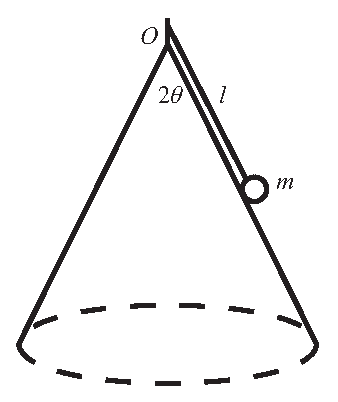
\includegraphics[scale=0.6]{C2-fig1.eps}
			\caption{作业T13题图}
			\label{C2-fig1}
		\end{minipage}
		\begin{minipage}[t]{0.48\textwidth}
			\centering
			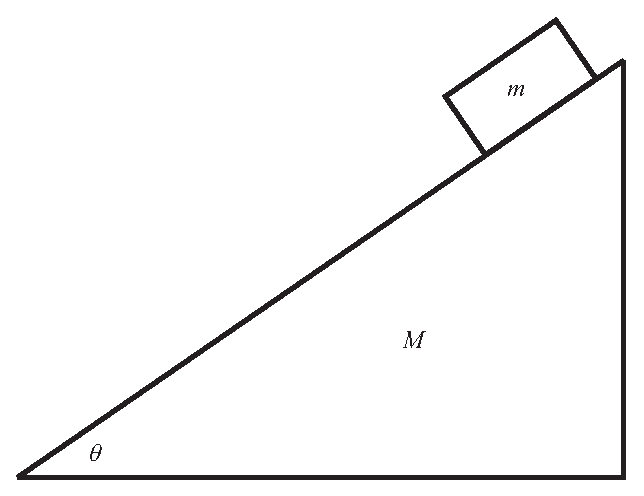
\includegraphics[scale=0.5]{C2-fig2.eps}
			\caption{作业T1题图}
			\label{C2-fig2}
		\end{minipage}
	\end{figure}
	
\end{enumerate}

\subsubsection{突撤约束}

\begin{enumerate}
	
	\item (作业T11) 两相同物体$A$和$B$分别固定在质量可以不计的弹簧两端, 竖直放在光滑水平支持面$C$上, 如图(\ref{C2-fig3})所示. 若把支持面$C$迅速抽走, 则在抽走的一瞬间, $A$的加速度大小 \uline{$a_A = 0$}, $B$的加速度大小 \uline{$a_B = 2g$}. 
	
	\item (作业T19) 如图(\ref{C2-fig4})所示, 一质量为$m$的小球被两个相同的弹簧拴住, 做向上匀速直线运动, 如果一根弹簧突然断掉, 则小球此时 \uline{加速度为$g/2$, 方向为竖直向下}. 
	
	\begin{figure}[H]
		\centering
		\begin{minipage}[t]{0.48\textwidth}
			\centering
			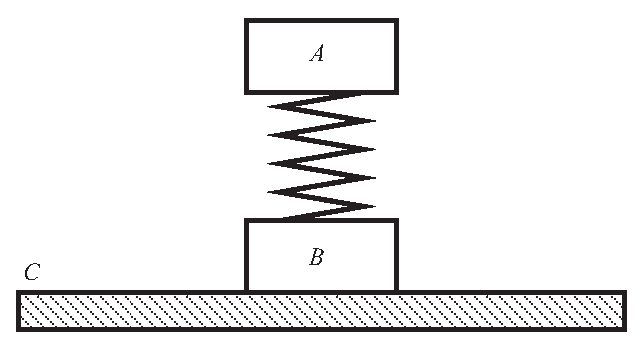
\includegraphics[scale=0.6]{C2-fig3.eps}
			\caption{作业T11题图}
			\label{C2-fig3}
		\end{minipage}
		\begin{minipage}[t]{0.48\textwidth}
			\centering
			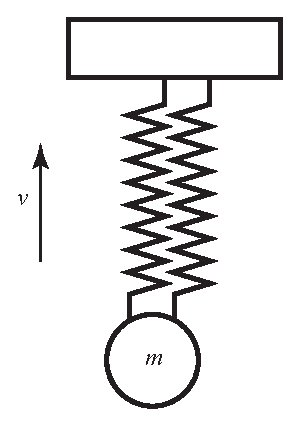
\includegraphics[scale=0.6]{C2-fig4.eps}
			\caption{作业T14题图}
			\label{C2-fig4}
		\end{minipage}
	\end{figure}
	
\end{enumerate}

\newpage
